% Chapter Template

\chapter{Preliminary Results} % Main chapter title

\label{ch:results} % Change X to a consecutive number; for referencing this chapter elsewhere, use \ref{ChapterX}

\lhead{Chapter 4. \emph{Results}} % Change X to a consecutive number; this is for the header on each page - perhaps a shortened title

We consider some results from applying the methods described in Chapter \ref{ch:methods} to the physical
models outlined in Chapter \ref{ch:models}, organized by model.
%----------------------------------------------------------------------------------------
%	SECTION 1
%----------------------------------------------------------------------------------------

\section{Polynomial Evaluations}
Using an analytic polynomial evaluation as our model allows observation of best-case performance of SCgPC for
several dimension cardinalities.  Uniformly distributing from 0 to 1, the mean and variance are
\begin{align}
  \text{mean}&=\left(\frac{3}{2}\right)^N,\\
  \text{var}&=\left(\frac{7}{3}\right)^N-\left(\frac{3}{2}\right)^{2N},
\end{align}
where $N$ is the cardinality of the input space.  As seen in Figures \ref{fig:anl5_varconv} and
\ref{fig:anl5_varconv}, the increase in dimensionality has great impact on the convergence rate of SCgPC
methods, but their exponential convergence eventually does beat out Monte Carlo.  Also of interest is the
adaptive methods.  In the figures, \emph{adapt} refers to adaptive Legendre quadrature sparse grid, while
\emph{adapt\_cc} refers to adaptive Clenshaw Curtis sparse grid.  While Legendre quadrature is traditionally
considered ideal for polynomial fitting, the Clenshaw Curtis quadrature seems to perform very similarly due to
the benefit of nested quadrature points.

\begin{figure}[H]
  \centering
    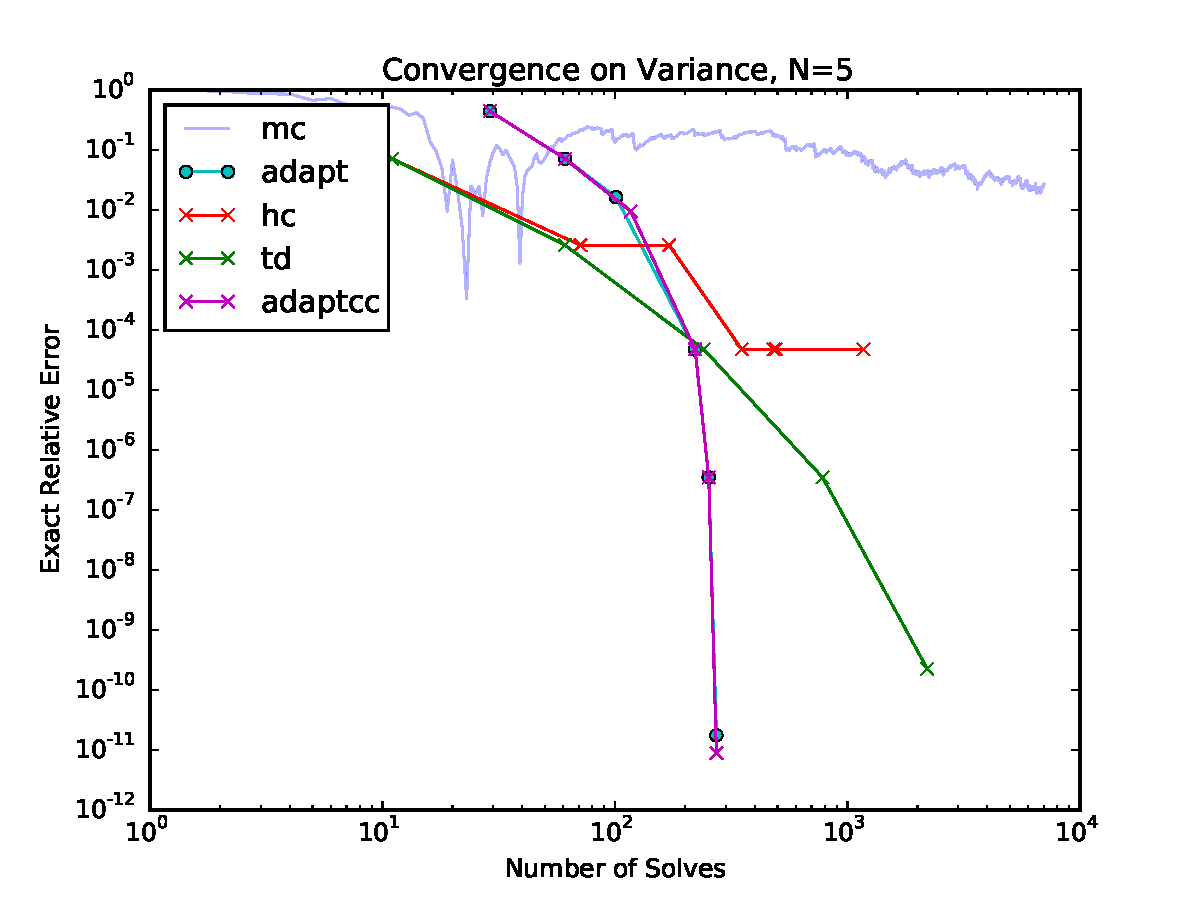
\includegraphics[width=0.7\linewidth]{./analytic5/anl_rand_varconv_5}
    \rule{35em}{0.5pt}
  \caption{Analytic $N=5$ Error Convergence, Variance}
  \label{fig:anl5_varconv}
\end{figure}
\begin{figure}[H]
  \centering
    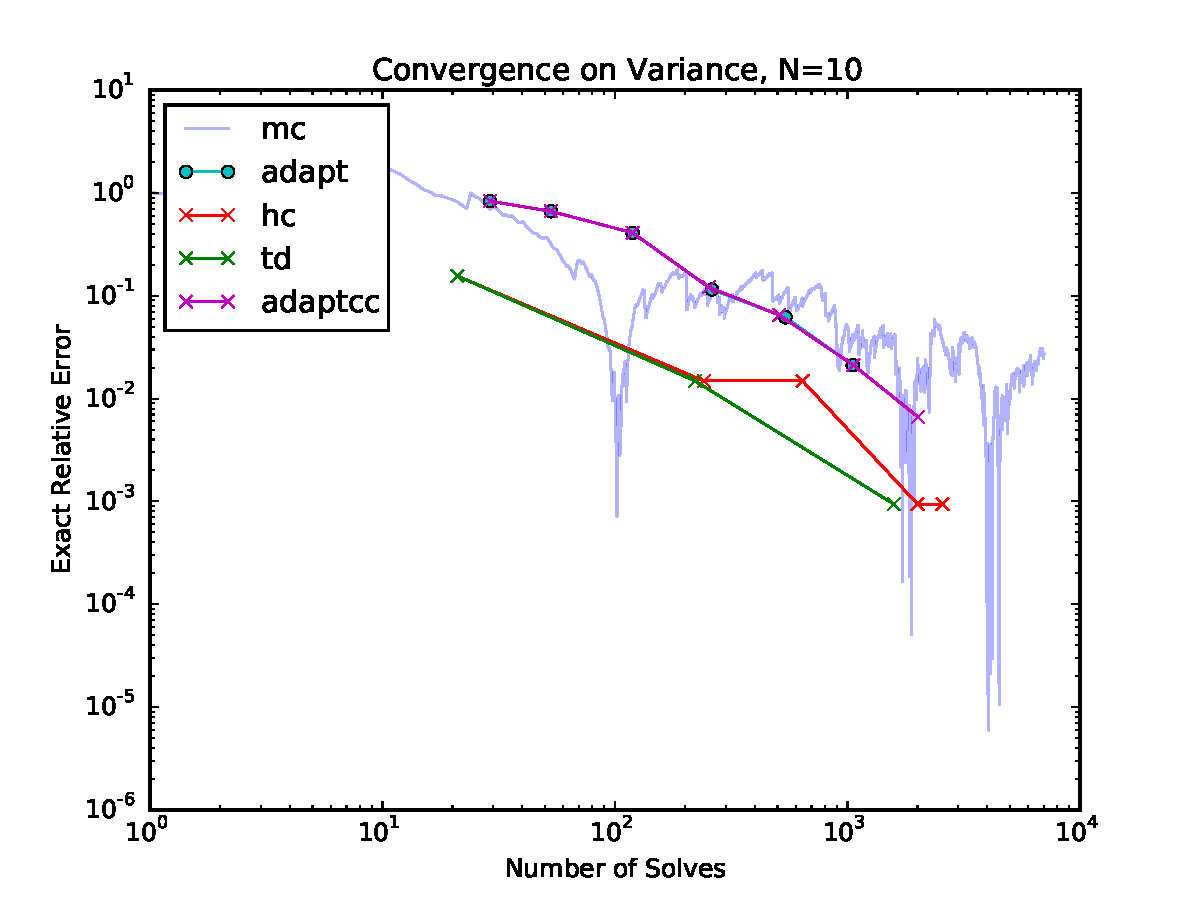
\includegraphics[width=0.7\linewidth]{./analytic10/anl_rand_varconv_10}
    \rule{35em}{0.5pt}
  \caption{Analytic $N=10$ Error Convergence, Variance}
  \label{fig:anl10_varconv}
\end{figure}



\section{Attenuation}
Similar to the polynomial model, the attenuation model does not converge exactly for any order of SCgPC
expansion, as exponential terms cannot be perfectly represented by a finite sum of polynomials.
Again distributing the input variables from 0 to 1, the mean and variance are
\begin{align}
  \text{mean}&=N^N\left(1-\exp(-\frac{1}{N})\right)^N,\\
  \text{var}&=\left(\frac{N}{2}\right)^N \left(1-\exp(-\frac{2}{N})\right)^N - \text{mean}^2,
\end{align}
where $N$ is the cardinality of the input space.  The convergence plots are shown in Figs.
\ref{fig:att5_varconv} and \ref{fig:att10_varconv}.
Interestingly, while the convergence of the adaptive method seems to be converging at a better rate than the
total degree isotropic set, there is no clear advantage for up to thousands of solves.  This is somewhat
expected, as there is little coupling between inputs in the attenuation model.  As with the polynomial model,
the curse of dimensionality is clear.

\begin{figure}[H]
  \centering
    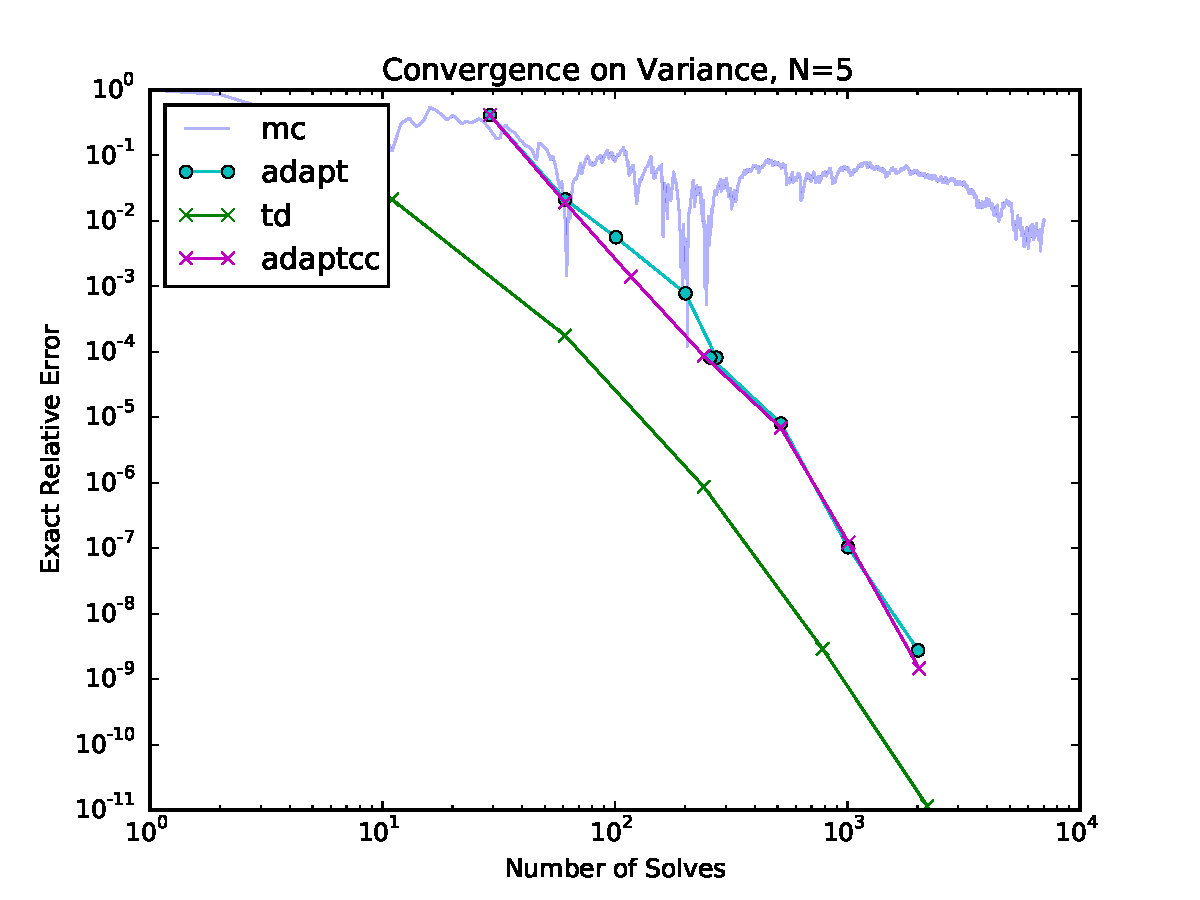
\includegraphics[width=0.7\linewidth]{attn_varconv_5}
    \rule{35em}{0.5pt}
  \caption{Attenuation $N=5$ Error Convergence, Variance}
  \label{fig:att5_varconv}
\end{figure}

\begin{figure}[H]
  \centering
    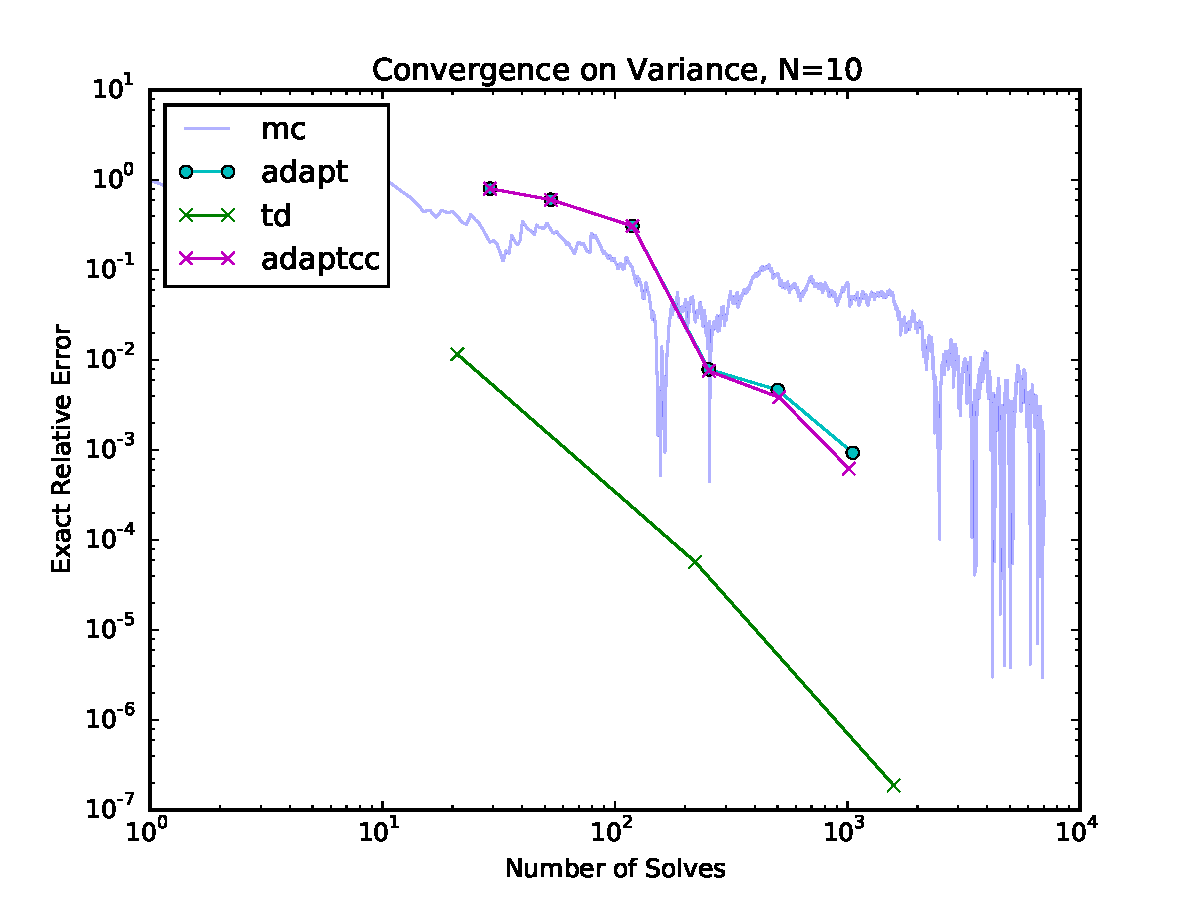
\includegraphics[width=0.7\linewidth]{attn_varconv_10}
    \rule{35em}{0.5pt}
  \caption{Attenuation $N=10$ Error Convergence, Variance}
  \label{fig:att10_varconv}
\end{figure}



\section{Projectile}
Unlike the attenuation and polynomial models, the projectile model is a nonlinear problem without an analytic
solution.  As a result, the convergence benchmark is one achieved by a large Monte Carlo run, instead of an
analytic benchmark; thus, the convergence of the various methods is limited to the convergence of the Monte
Carlo point.  The most converged Monte Carlo point for this work is
\begin{align}
  \text{mean} = 1234, \\
  \text{var} = 1234.
\end{align}
Additionally, this is the first model where significant anisotropy exists in the model.  For instance, the
drag coefficient parameter is many orders of magnitude more influential on the quantity of interest than the
gravitational acceleration.  
The results in Fig. \ref{fig:proj_varconv} are interesting, and require additional data points to understand
clearly.  However, we include Fig. \ref{fig:proj_varval} for clarity.  While it initially looks like the adaptive
methods converge quickly, it appears that this is misleading, as shown in the values graph.  The adaptive
method is converging, but passes through the benchmark value before turning back to converge on it.  This
indicates the adaptive construction introduces too much variance initially, and additional terms are required
to approach the benchmark solution.
\begin{figure}[H]
  \centering
    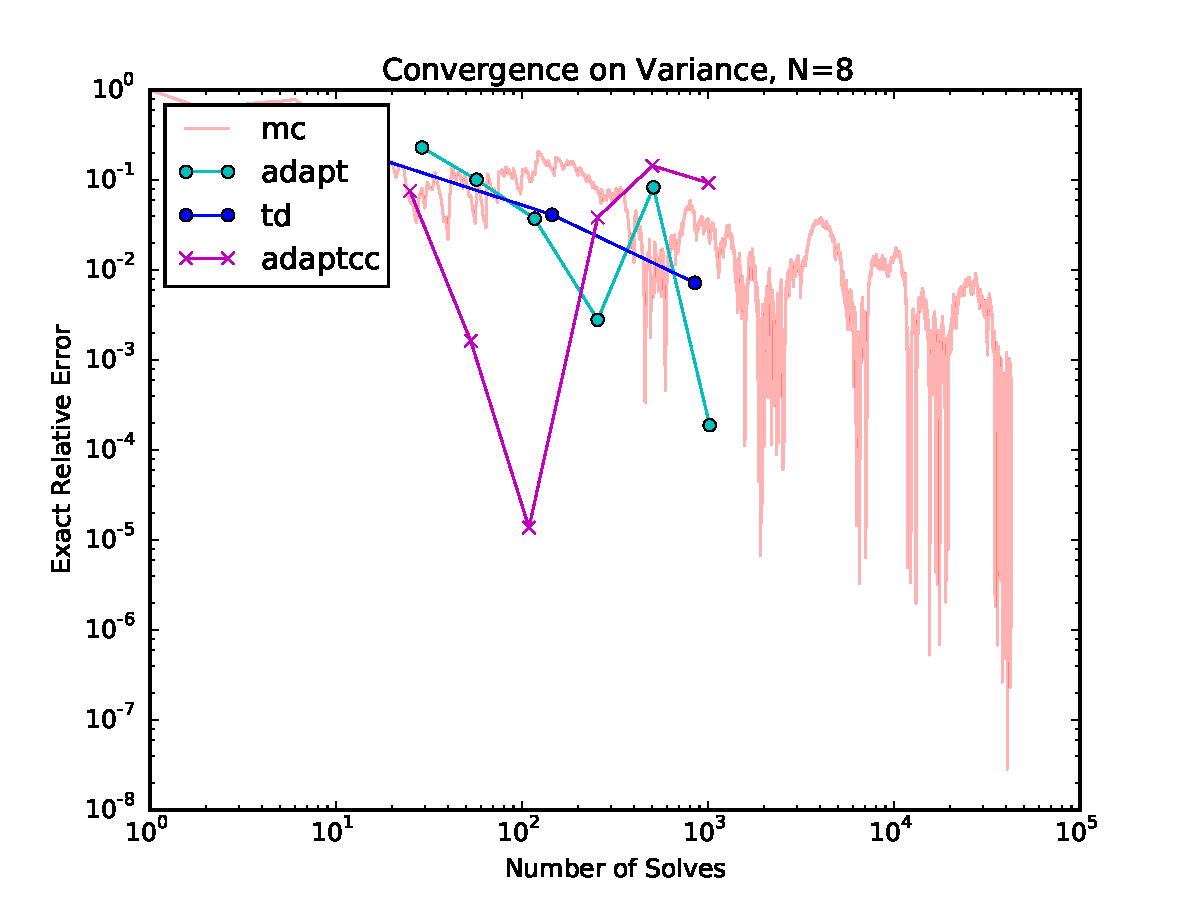
\includegraphics[width=0.7\linewidth]{proj_varconv_8}
    \rule{35em}{0.5pt}
  \caption{Projectile $N=8$ Error Convergence, Variance}
  \label{fig:proj_varconv}
\end{figure}
\begin{figure}[H]
  \centering
    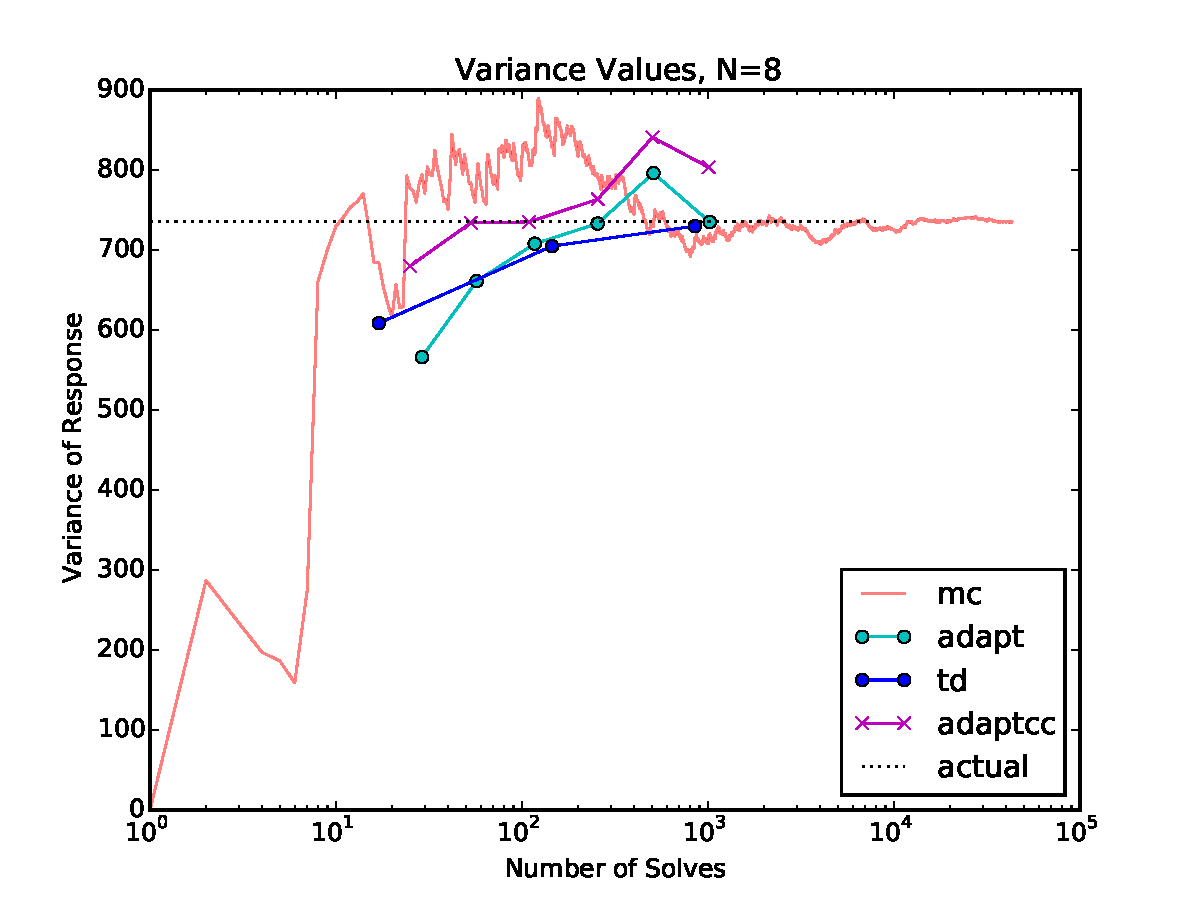
\includegraphics[width=0.7\linewidth]{proj_varvals_8}
    \rule{35em}{0.5pt}
  \caption{Projectile $N=8$ Values, Variance}
  \label{fig:proj_varval}
\end{figure}
%\begin{figure}[H]
% \centering
%   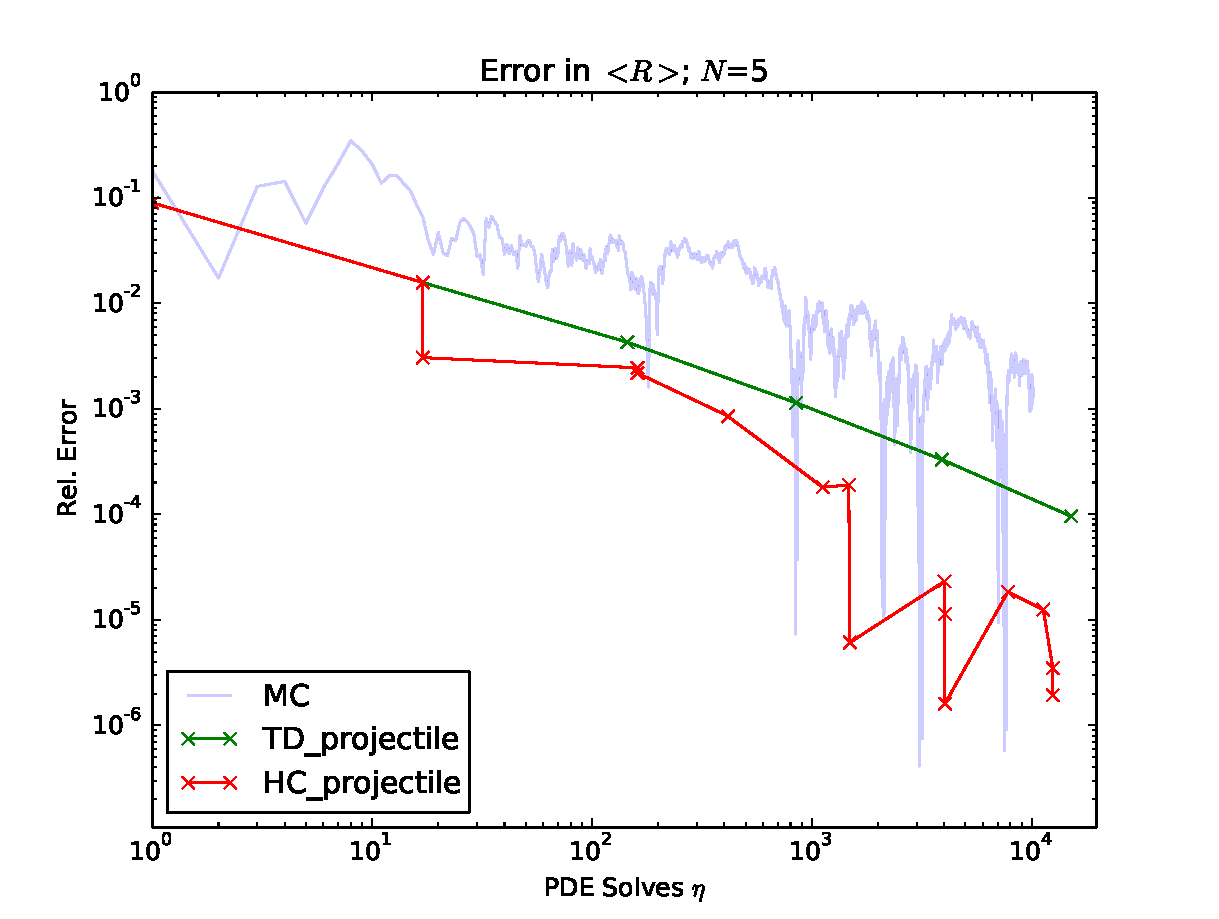
\includegraphics[width=0.7\linewidth]{projectile_errs}
%    \rule{35em}{0.5pt}
%  \caption{Projectile $N=8$ Error Convergence, Variance}
%  \label{fig:proj_varconv}
%\end{figure}



\section{Neutron Diffusion}
The neutron diffusion model is a complex, nonlinear model that begins to approach an engineering-scale model.
Because of complications with conflicting libraries, the adaptive SCgPC method was not available for this
model.  Particularly of note is the clear and obvious loss of convergence rate with increase in the
cardinality of the input space. \{Note to self: fix coloring in plots.\}

\begin{figure}[H]
  \centering
    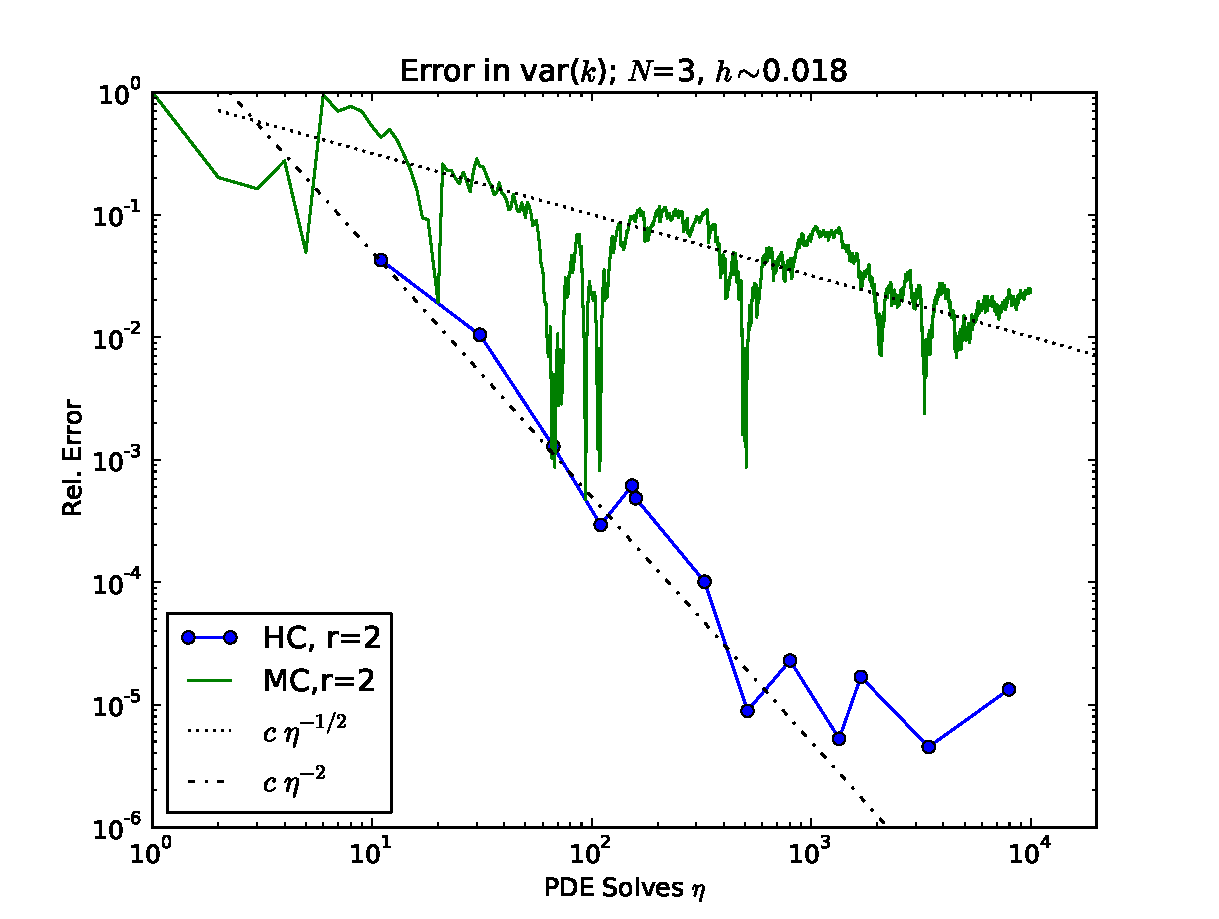
\includegraphics[width=0.7\linewidth]{N3_h5_MCHC_2}
    \rule{35em}{0.5pt}
  \caption{Diffusion $N=3$ Error Convergence, Variance}
  \label{fig:diff3_varconv}
\end{figure}
\begin{figure}[H]
  \centering
    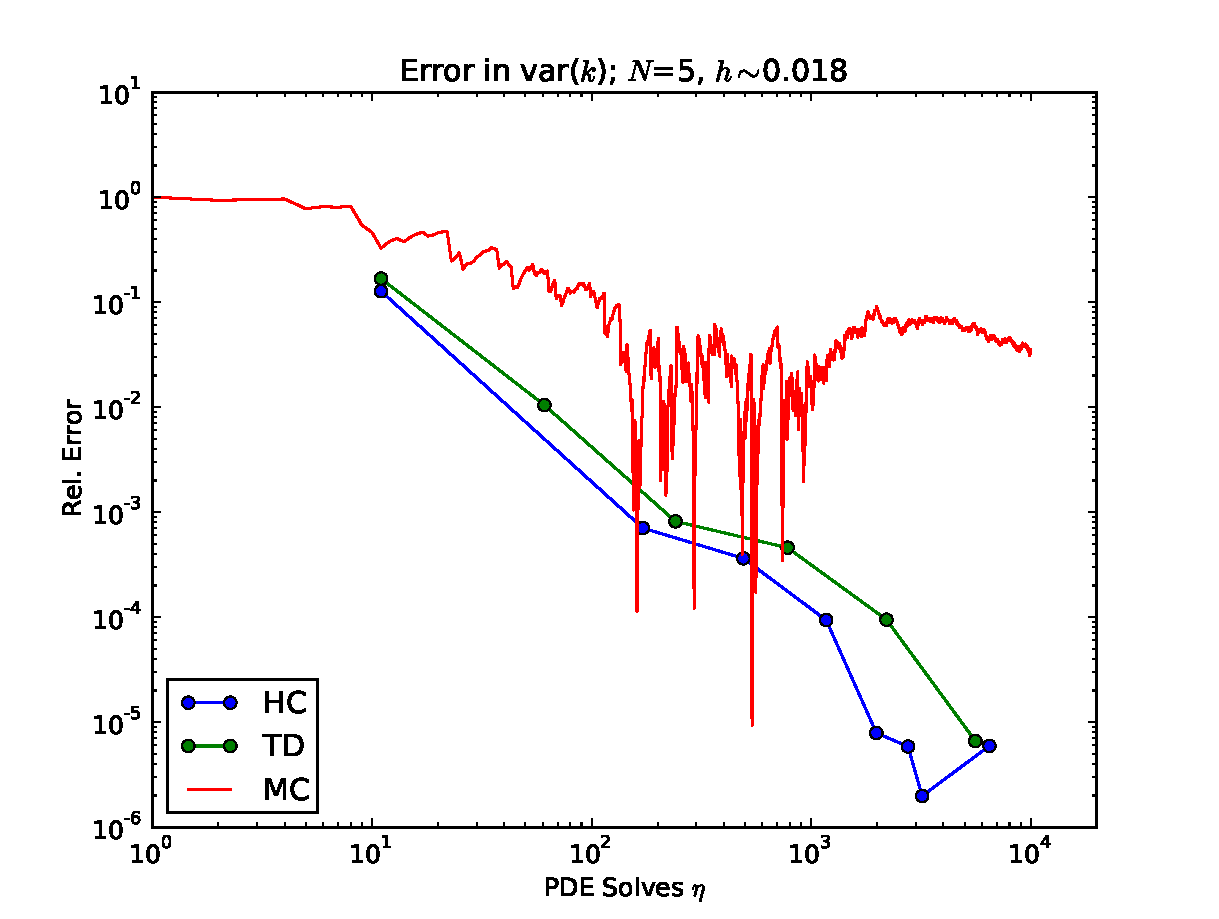
\includegraphics[width=0.7\linewidth]{N5_h5_MCHC_2}
    \rule{35em}{0.5pt}
  \caption{Diffusion $N=5$ Error Convergence, Variance}
  \label{fig:diff5_varconv}
\end{figure}
\begin{figure}[H]
  \centering
    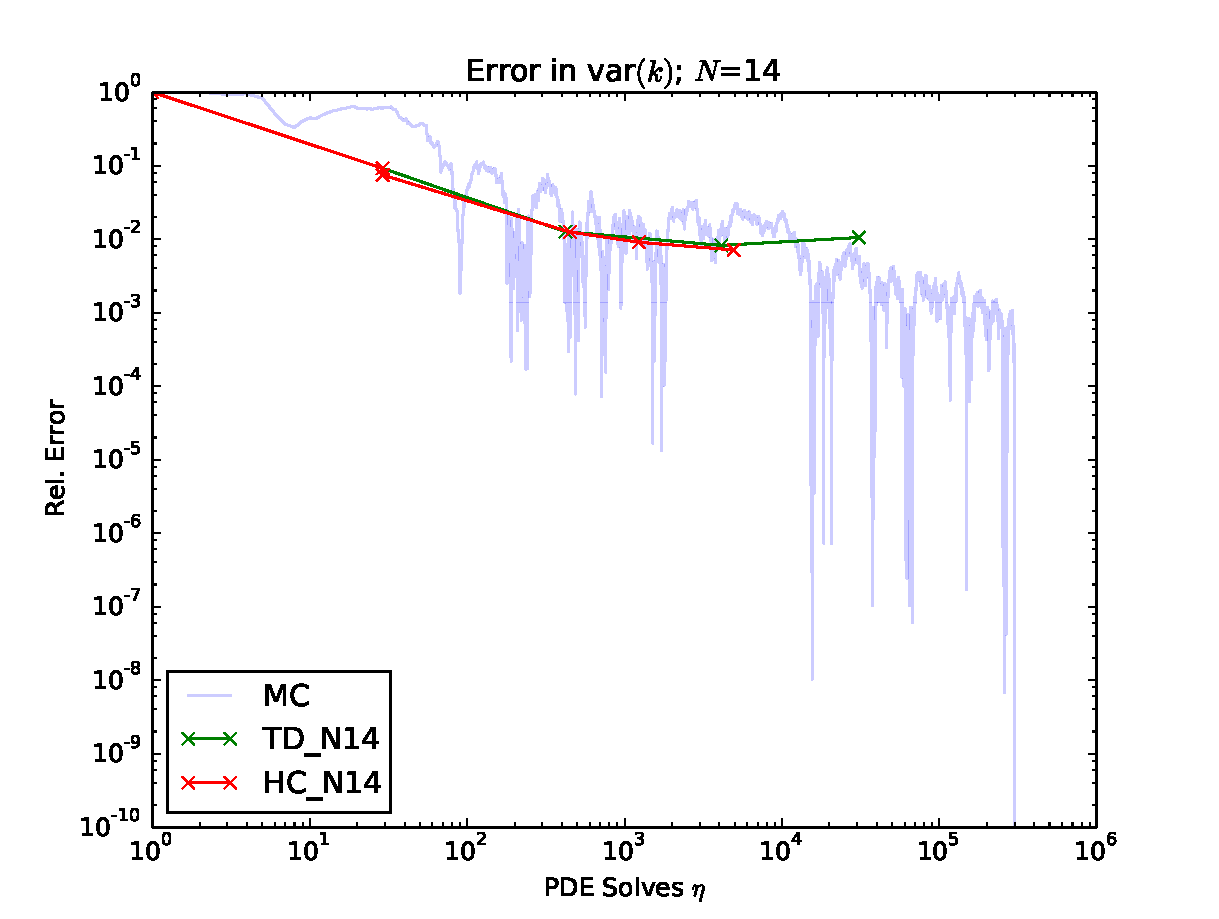
\includegraphics[width=0.7\linewidth]{N14_iso_var_errs}
    \rule{35em}{0.5pt}
  \caption{Diffusion $N=14$ Error Convergence, Variance}
  \label{fig:diff14_varconv}
\end{figure}





\section{Fuel Rod Performance}
Because of non-deterministic failures in BISON, insufficient data has been collected to present convergence
plots for this model.


\section{Conclusions}
From evaluating the results using the various methods on these models, there are a few useful conclusions.

First, especially for models with small input cardinality, SCgPC methods tend to be faster converging than
traditional Monte Carlo methods.  In particular, the adaptive SCgPC method eventually exhibits exponential
convergence in the models considered here.  This is encouraging for many uncertainty quantification problems
where the variance is chiefly centered on a few input parameters.

Second, using Clenshaw Curtis quadrature appears to have no negative consequence on converging with the
adaptive SCgPC method, but no striking positive consequence either.  This suggests it is worth exploring other
nested quadrature methods that might be beneficial in general, or at least in certain circumstances.

Third, it is clear that even with adaptive SCgPC, convergence is poor for input spaces with more than a dozen
inputs for less than a thousand solves.  For costly engineering codes, even a thousand runs may be
impractical, so further improvement of the adaptive algorithm is necessary.  This leads to the desirability of
the adaptive HDMR method, which can further subdivide the input domain.  These subdivided domains have
cardinality much more suitable to SCgPC methods.

Lastly, because SCgPC methods improve drastically with decreases in input cardinality, we expect SCgPC to
benefit from coupling with input reduction methods, such as sensitivity-weighted input reduction through
principal component analysis using input-input covariance matrices.
